The proposed implementation of the ECDAR code generator is split up
in two parts. The first part is a framework of abstract classes, implementing
in as much detail as possible the single parts of ECDAR specifications
(i.e. edges, locations, TIOA). The second is the actual code generation.
Our code generator generates source code which inherit from the abstract
framework to minimize the amount of code that needs to be
generated. This means that nearly all design decisions have been made
prior to generating code, reducing space for possible errors. This
section describes our implemented subset of ECDAR and the code generator
in detail.

\subsection{Tasks}
\label{subsec:tasks}

ECDAR defines the behavior of a system as a state machine. This behavior
is, however, still too abstract to justify code generation. We can
generate code which implements the behavior of state machines, but
in essence, the system would then only produce messages.

To make this tool more useful, we introduce the notion of tasks as an extension
to the language. Each location is assigned exactly one task. A task is a
procedure which will be executed as soon as an automaton traverses over an edge,
arriving at a new location. Such a task could for example be a procedure that
heats up the water in the coffe machine from Fig. \ref{bev-machine} or some code
that extends the undercarriage of a plane when approaching the landing strip.

Tasks can either be preemptive or non-preemptive. This property becomes
important for defining behavior of automata when they are notified
about input by the controller.

ECDAR is input-enabled (see Sect. \ref{introduction-ecdar}) and therefore,
the system is required to react to input immediately. As a consequence,
there must also be a well defined reaction to input during the execution
of a task.

When an automaton is executing a task and it receives an input message
which it accepts, it may stop the currently executed task and proceed
as originally defined in ECDAR (i.e. traverse the corresponding edge),
if and only if the task is preemptive. Otherwise, the given input
will be ignored and the execution of the task continues.

To determine if a task is preemptive is up to the designer of the
system to decide. By default all tasks are non-preemptive.

\subsection{The ECDAR Framework}
\label{implementation-framework}

\begin{figure}[t]
\begin{centering}
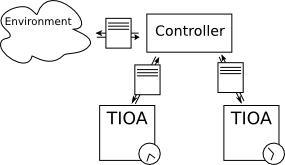
\includegraphics[scale=0.8]{images/ecdar_architecture_2.png}
\par\end{centering}

\caption{Schematic of the architecture of our ECDAR implementation.}
\end{figure}

The architecture we chose is based upon the work of Amnell et
al.\cite{amnell_code_2002} with some modifications. Communication between
automata is implemented as message passing between a controller and automata,
where automata send messages to the controller by traversing over output
edges. This is different in actual ECDAR, where automata communicate through
message passing directly between each other. However, by choosing a slightly
different architecture, we can unify the message system in the implementation,
handling all messages central and also not distinguishing between a message
coming from the environment or a message send by an automaton. The resulting
behavior is equal.

Automata need to execute in quasi-parallel. In the implementation they are run
in a classical threading architecture that does not require multiple processor
units. Since there is no communication between automata directly, we can
minimize synchronizing between threads (see more on synchronizing in
Sec. \ref{subsec:synch}).

The following overview will give further implementation details on each
component of ECDAR as we implemented it. Each component is illustrated with a
short code example, implementing ECDAR's ``University''
example\footnote{\url{http://people.cs.aau.dk/adavid/ecdar/examples.html#university}}. For
clarity, we omit the framework implementation and focus on the generated code.

\subsubsection{Controller.}

\begin{figure}[t]
\lstinputlisting[linerange={6-11,63-63}]{../dk.itu.ecdar.text.generator.mockup/src/dk/itu/ecdar/text/generator/mockup/university/UniversityController.java}
\caption{Example of controller code.}
\label{controller-example}
\end{figure}

The controller holds all automata given in the specification and notifies them
about received messages. It is a singleton, accessible in a static fashion.
This property is useful for sending messages to the controller.

\subsubsection{TIOA.}

The implementation of timed I/O automata holds a set of locations and a
reference to the location it is currently at. The TIOA is executed by a thread
that keeps checking for available edges and traverses along these as soon as
they become enabled. To check if an edge is available, let $E_{s\rightarrow t}$
be an edge where $s,\, t$ are start and target locations
respectively. Furthermore, let $g(E)$ be a function evaluating the guard of an
edge $E$ and $I(l)$ a function evaluating the invariant of a location $l$. Our
implementation uses $g'(E_{s\rightarrow t})=g(E_{s\rightarrow t})\wedge I(t)$ to
check if $E_{s\rightarrow t}$ is available. We do not check the invariant of the
source location because if the source location's invariant was violated, the
system would already be in a deadlock. This cannot be true, as we assume that
the system is verified.

\begin{figure}[t]
\lstinputlisting[linerange={8-8,157-170}]{../dk.itu.ecdar.text.generator.mockup/src/dk/itu/ecdar/text/generator/mockup/university/Machine.java}
\caption{Example of TIOA code.}
\label{tioa-example}
\end{figure}

Additionally, the automaton has the ability to return the current
local clock state (see \ref{implementation-presumptions}) and to
reset the clock. We use the same notion of clocks as \cite{amnell_code_2002},
where time on the local clock is the difference between the current
time on the system clock and the time the local clock was started.
Resetting the local clock means to use the current system clock time
as the new start time (see Fig. \ref{tioa-example}).

\subsubsection{Locations.}

\begin{figure}[t]
\lstinputlisting[linerange={98-119}]{../dk.itu.ecdar.text.generator.mockup/src/dk/itu/ecdar/text/generator/mockup/university/Machine.java}
\caption{Example of location code.}
\label{location-example}
\end{figure}

Each location is associated with a task (see Sec. \ref{subsec:tasks}). Task
execution is implemented in a separate thread so that the execution of the
automaton is never blocked. Locations are implemented as objects holding an
array of edges that point away from it. (See Fig. \ref{location-example})


\subsubsection{Edges.}
\label{subsubsec:edges}

\begin{figure}[t]
\lstinputlisting[linerange={11-24}]{../dk.itu.ecdar.text.generator.mockup/src/dk/itu/ecdar/text/generator/mockup/university/Machine.java}
\caption{Example of edge code.}
\label{edge-example}
\end{figure}

An edge holds a reference to the location which the parent automaton
will be at after traversing this very edge. Edges can be asked if
they will be available at a given time. This is implemented to enable
lazy waiting in the automaton's traversal checker. Each edge is associated
with some input. If an edge is controllable, it will be triggered
if the automaton is notified at this input. If it is uncontrollable,
it will send its input to the controller. Furthermore, edges have
access to the clock of the parent automaton to reset it appropriately.

The implementation makes a class-wise distinction between input edges
(i.e. edges that are traversed when a corresponding message was received) and
output edges (edges that send messages on traversal) and hard-codes the behavior
in the framework, e.g. messaging the controller (see Fig. \ref{edge-example}).



\subsection{Synchronization}
\label{subsec:synch}

In the framework implementation, the Java keyword \textit{synchronized} is 
used for making certain operations quasi-atomic. That means, that a set of
instructions may not be interrupted by the execution of another thread -- 
i.e. traversals over edges.

This is mainly used for the logging of signals, so that logging time
is preserved and the output appears in the right order. \textit{Synchronized}
is also used, to set some internal states on TIOA, where the internal state
consists of multiple values that need to be set at the same time.

\textit{Synchronized} is furthermore used to prioritize handling of input.  The
method on the controller object, that is handling the signal, as well as those
on the TIOA that react to a signal if it is accepted, are modified with
\textit{synchronized}. This ensures that, before everything else, the input is
processed.


\subsection{Code Generation}
\label{implementation-code-generation}

In the implementation the generation of source code is done
through a model to text transformation. The generation outputs compilable
Java based on input from an ECDAR file.

The Eclipse Modeling Framework (EMF) is utilized for the process. EMF is a
modeling framework and code generation facility for building applications based
on a structured data model. From a model specification described in the XMI-format, EMF
provides tools and run time support to produce a set of Java classes for the
model, along with a set of adapter classes that enable viewing and command-based
editing of the model and it provides a basic editor. The core EMF framework
includes a meta model -in Ecore- for describing models and run time support for the
models including: change notification, persistence support with default XMI
serialization, and a very efficient reflective API for manipulating EMF objects
generically. In the implementation presented in this paper an Xtext environment
is generated from the ECDAR Ecore model. Xtext is a framework for development of
programming languages and domain specific languages.

In order to generate code from the model it's imperative to follow a process of
multiple steps: Get the input from ECDAR, translate this to Xtext ECDAR DSL,
setup a workflow that manages the process and finally a Xpand-template is needed
to define how the transformation output should look like. Each step is described in more detail in the following section.

\subsubsection{Transformation Process}
\label{transformation-process}

The initial output from the ECDAR tool is in XML-format. The XML-output
contains a complete definition of the model with locations, edges, variables,
transformations etc. In order to work with these files and do the actual code
generation, a conversion to Xtext ECDAR DSL is needed. For this conversion we
are using a converter (courtesy of Bastian M\"uller) that simply takes the ECDAR XML-file and converts it to ECDAR DSL. The ECDAR DSL syntax is defined in our Xtext ECDAR
environment. With the combination of the Ecore meta model and the Xtext syntax a
workflow can be defined. This workflow is describing how to handle the
generation process. This is done with the help of the ``Modeling Workflow Engine 2''
(MWE2). Also referenced in the workflow is the template that describes how the
actual output is going to look like. The templates are written using
Xpand. Xpand is a statically typed template language. Conveniently Xpand
supports code-completion directly connected to the Ecore model defined in the
MWE2 workflow, but also comes with syntax coloring, refactoring and error
highlighting. The output generation results, for the system presented in this
paper, are based on several workflows and templates to do the rather complex
transformations: One set of workflows and templates for respectively the
Specification, Controller and Environment.

More specifically in the workflow-file one defines what model to use, a
slot-name to refer to later and an entry point. The entry point defines which
class element is the top or root element. The entry-element that is specified for
the three aforementioned workflows is "ETSpecificationDefinition". Also defined
in the workflow is how to use the entry-element. For instance in the
specification workflow it is defined that for each "ETSpecificationDefinition" a
transformation is done using the Xpand template for this particular
generation. The end result is generated output for each specification that
was initially described and modeled from within the ECDAR XML-file.

With the workflow fully configured, the next step is to write the
transformation. This is done in a Xpand template. The snippets in Fig.
\ref{xpand-example} shows some important steps.

\begin{figure}[t]
\lstinputlisting[linerange={1-2}]{code/TemplateSpecifications.xpt}
\lstinputlisting[linerange={6-6}]{code/TemplateSpecifications.xpt}
\lstinputlisting[linerange={34-41}]{code/TemplateSpecifications.xpt}
\caption{Snippets from Xpand-template \label{xpand-example}}
\end{figure}

The arrows, known as guillemots (``\guillemotleft'' and ``\guillemotright''),
indicates where in figure \ref{xpand-example} the XPAND language is in place. First
of all an import of the model is done in the first line, referenced as
ecdarText. We then proceed to one of the central concepts of Xpand by using the
define-block; This is where we define our template. We only use one template in
this specific file, but it could have contained multiple, which would have
resulted in multiple define-blocks. In the next and last snippet we jump to a
part where we are iterating through each edge and create a constructor for the
current class. In the first line we create the constructor by inserting the text
"Edge" and add the number the iterator has reached. We then iterate through a
list of the current Edges variables, which should be one signal, and returns the
results as a list. We furthermore use a new iterator to keep track of this
iteration. Afterward we use a check too make sure it's the first iteration, and if it is, we
print out the current Edge target name and the variable signal, such as "super(C,
"signal");".

The notion of tasks as previous described in section 3.2. is accounted for in
our generated output. In the controller we generate functions that will be
invoked at each location. A task is a procedure which will be executed as soon
as an automaton traverses over an edge, arriving at a new location. There can
only be one task for each location. The idea behind having all methods in the
controller is for a better overview and a centralized customizable file.

